\section{The waveform forward model and its calibration}\label{sec:model}
\sectionstate{ready}{\texttt{WAVEFORM\_FIRST\_THREADING.md} \S4, \S9, \S15; \texttt{wft/}; R9 (calibration protocol)}
\intent{The model (per-plane pulse template, sharing kernel, drift and diffusion), the fit, and the calibration
protocol with its traps: per detector and per run condition; kernel ordering enforced
(\texttt{check\_kernel\_ordering}); $v$ from the kernel hyperfit, never from a Magboltz prior; cut units that move with $v$.}
\analysis{R9}{collect the protocol and the traps from WFT \S15, RETIRE\_C2GTC1, the in-situ findings}
\tbw{Frozen calibration (C2, 2026-10-23): the physical RC kernel --- prompt footprint $\sigma_0$ per view
($\sigma_{0,x}\approx0.25$\,mm, the physical value: strip integration 0.225\,mm alone; the head-on stacks' 0.35--0.43
also carry the asymmetric neighbour copy), RC spread $D_\mathrm{rc}$ along the resistive strips, drift diffusion; no
fitted copy amplitudes. $v$ fitted with the reference position profiled (a reference taken from a hit-time alignment
biases $v$ by 3--15\,\%). The delay kernel (r06) is the comparison.}
\tbw{Main known mismatch: the model is symmetric in X, the June boards are not~\cite{paperI}. It shows as the X
$\chi^2$ structure and the $\sigma_{0,x}$ tension between per-event fits and stacks. Cost (toy, \S\ref{sec:floor}):
$-0.05$\textdegree{} overall, $\mp0.19$\textdegree{} head-on, $+0.007$\textdegree{} on the resolution. Not modelled: no
mechanism makes its size, so a term would be a free parameter per board and per run condition.}
\begin{figure}[t]
  \centering
  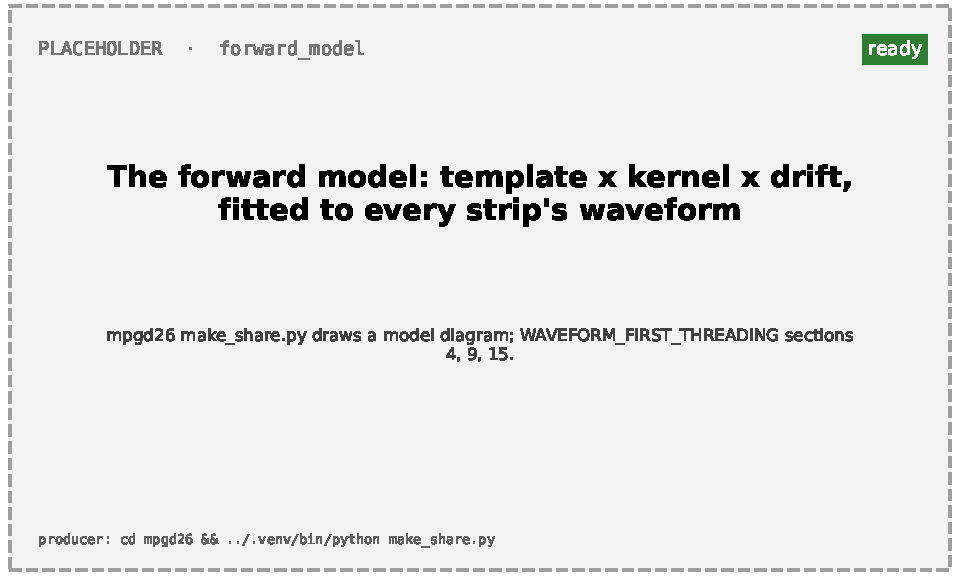
\includegraphics[width=0.9\linewidth]{forward_model}
  \caption{\tbw{The forward model.}}
  \label{fig:forward_model}
\end{figure}
